\newcommand{\subject}[1]{\renewcommand{\subject}{#1}}
\newcommand{\keywords}[1]{\renewcommand{\keywords}{#1}}

\documentclass[twocolumn]{article}

\date{\today}
\subject{Chemistry}
\keywords{Spin Casting, Polymers, Polystyrene, Molecular Weight.}

\usepackage{docstyle}
\setlength{\columnsep}{1cm}
\usepackage[affil-it]{authblk}
\usepackage{caption}
\usepackage[version=4]{mhchem}
\usepackage{siunitx}
\usepackage{xurl}
\usepackage{amsmath}
\usepackage[style=chem-acs]{biblatex}
\usepackage{booktabs}
\usepackage{pgfplots}
\usepackage{float}

\bibliography{savedrecs}

\title{\bfseries Spin Casting to Confirm the Molecular Weight of a Polystyrene Sample}

\author{Samuel~Coopersmith}
\affil{Casa Grande High School}

\author{Brinley~Dai}
\affil{The Experimental High School Attached to Beijing Normal University}

\author{Sahana~Dhama}
\affil{The Wheatley School}

\author{Peter~Elmer}
\affil{High School for Math, Science and Engineering}

\author{Dylan~Fei}
\affil{Jericho Senior High School}

\author{Hannah~Feng}
\affil{Torrey Pines High School}

\author{Anita~Gaenko}
\affil{Huron High School}

\author{Jerry~Gao}
\affil{Beijing No.~80 High School}

\author{Jacqueline~Han}
\affil{Great Neck South High School}

\author{Anna~Heimowitz}
\affil{Stella K.~Abraham High School}

\author{Sharis~Hsu}
\affil{Valley Christian High School}

\author{Ellen~Hu}
\affil{C.~Leon King High School}

\date{}

\begin{document}
	\maketitle
    \begin{abstract}
        Molecular weight is crucial to characterizing and understanding polymers. Using molecular weight, we can approximate the length of the polymer chains in a polystyrene (PS) sample, thereby allowing us to predict properties of the polymer. In this experiment, spin casting and ellipsometry were utilized to find the molecular weight of a  pure PS sample ($M_\text{w} = $ \qty{280000}{\atomicmassunit}) was applied and tested. Employing fourier-transform infrared spectroscopy (FTIR), differential scanning calorimetry (DSC), UV-visible spectrometry, and goniometry, the sample was confirmed to be PS.\@ FTIR analysis confirmed that the sample was pure PS, while DSC determined the glass transition temperature to be \qty{107.41}{\degreeCelsius}, in agreement with reported PS values. 
        
        The sample was then dissolved in various concentrations ranging from \qty{25}{\milli\gram\per\milli\liter} to \qty{37.5}{\milli\gram\per\milli\liter} (in \qty{2.5}{\milli\gram\per\milli\liter} increments) and spun cast on silicon wafer squares. The resulting PS-coated silicon wafers were measured via ellipsometry to determine thickness. Contact angles were determined via a goniometer for both PS-coated (\qty{82.52}{\degree}) and non-coated (\qty{15.12}{\degree}) wafers. PS-coated wafers were then exposed to UV/Ozone, and the contact angles were measured, corroborating industrial processes of creating hydrophilic PS materials. 
        
        The findings support previous experiments that use spin-casting to infer\slash deduce the molecular weight of polystyrene samples.
    \end{abstract}

        \section{Introduction}
        Polystyrene (PS), an aromatic polymer, is formed by the polymerization of styrene monomers\autocite{WOS:Weith}. Polystyrene finds extensive application in various sectors, most prominently in the food industry\autocite{WOS:Paraskevopoulou}. There, it is used to package food items in the form of lids, and converted into foam to make cups, containers, trays, etc. This is because it is low in cost, light weight (as foam), easy to process, and hydrophobic\autocite{WOS:He}. In research, polystyrene is utilized to produce instruments like test tubes and tissue culture trays.\autocite{WOS:Lerman} Evaluating the molecular weight of polystyrene can provide valuable insights into its mechanical properties, such as polymer chain length\autocite{WOS:Smirnova}. These properties encompass viscosity\autocite{WOS:Tang}, chemical resistance\autocite{WOS:Feng}, and facilitate efficient utilization of the polymer\autocite{WOS:Ismail, WOS:Zizkova, WOS:Siswosukarto, WOS:Motta}.

        One approach to determining the molecular weight involves spin-casting polystyrene solutions with different concentrations onto silicon (\ce{Si}) wafers. This technique yields thin layers of polystyrene characterized by high material purity, weight, and density\autocite{WOS:Dinelli}. To validate the accuracy of the spin-casting method, the molecular weight of a polystyrene 280K sample from Wafer World Inc.\ was determined in this experiment.
        
        The experiment aimed to accomplish five primary objectives:
        \begin{enumerate}
            \item Understanding the crystal structures of \ce{Si} wafers and processing \ce{Si} wafer surfaces.
            \item Spin-casting thin polymer films.
            \item Measuring the thickness of these films.
            \item Identifying various polystyrene characteristics.
            \item Confirming the molecular weight of a known polystyrene sample. 
        \end{enumerate}

        To achieve these objectives, a range of equipment and methodologies were employed, including the creation of a solution containing polystyrene and toluene, cleaving silicon wafers, utilizing an optical microscope, ultraviolet-visible spectroscopy (UV-Vis), differential scanning calorimetry (DSC), compression molding, Fourier-transform infrared (FTIR) spectroscopy, a spin caster, contact angle calculation, and an ellipsometer. These equipment and methodologies were categorized into three main sections: preparation, confirmation of polystyrene identity, and determination of molecular weight. 
        
        \section{Materials and Methods}
            \subsection{Silicon Cleaving}
            24 square Si(100) wafers were prepared, each of length \qty{1}{\centi\meter}. These wafers would serve as the substrates to the six polystyrene solutions, allowing us to use four wafers per concentration. Clean, undamaged silicon wafers were placed upon dry paper towels with its dull, non-smooth side facing up. Two holes that measured \qty{1}{\centi\meter} were cut between them, thereby facilitating the cutting process.
            
            The silicon wafer was then aligned with the pre-cut \qty{1}{\centi\meter} measurement, and from there, a diamond-tip cutter was used to carefully scrape vertically across the desired point, applying the most pressure at the edge (bottom- and top-most) parts of the wafer, while holding the whole piece of silicon in place using a tweezer. These cut silicon wafers were then placed in petri dishes and sealed with Parafilm grafting tape.

            Two options of silicon configurations on the Miller index were available: Si(100) and Si(111). These orientations differ in that the Si(100) configuration will produce crystals that cleave naturally into cubic structures whereas the Si(111) configuration will produce crystals that cleave naturally into triangular structures \qty{45}{\degree} (Figure \ref{fig:silicon}). Thus, because our experiment requires square wafers, we used Si(100) as opposed to Si(111).

            \begin{figure}
                \centering
                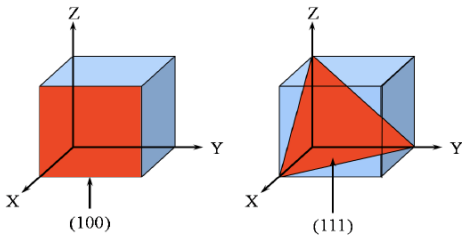
\includegraphics[width=0.8\columnwidth]{img/silicon.png}
                \caption{Possible slicing directions for (100) and (111) indices of silicon.}\label{fig:silicon}
            \end{figure}

            \subsection{Polystyrene Solutions}

                \begin{table}
                    \centering
                    \begin{tabular}{@{}ccc@{}}
                        \toprule
                        Soln. conc. (\unit{\milli\gram\per\milli\liter}) & PS mass (\unit{\milli\gram}) & Toluene vol (\unit{\milli\liter}) \\ \midrule
                        25.0                           & 69.9                  & 2.80                \\
                        27.5                           & 72.9                  & 2.62                \\
                        30.0                           & 87.7                  & 2.92                \\
                        32.5                           & 95.1                  & 2.93                \\
                        35.0                           & 98.8                  & 2.83                \\
                        37.5                           & 101.6                 & 2.71                \\ \bottomrule
                    \end{tabular}
                    \caption{List of PS solutions prepared.}\label{tab:soln}
                \end{table}

                Six concentrations of polystyrene in toluene were prepared, ranging from \qtyrange{25}{37.5}{\milli\gram\per\milli\liter} (incremented by \qty{2.5}{\milli\gram\per\milli\liter}). We chose to use 99.9\% toluene as the solvent for the polystyrene pellets ($M_\text{w} = $ \qty{280000}{\gram\per\mol}) due to its ability to easily dissolve organic solutes. We weighed six different masses of polystyrene 280K (error of \qty{\pm 0.01}{\milli\gram}) and, in turn, measured six different volumes of toluene (error of \qty{\pm 0.1}{\milli\liter}).

            \subsection{Spin Casting}
                Utilizing a Headway Research PWM 32 Spin Coater, thin layers of varying concentrations of polystyrene were coated onto the surface of silicon wafers. The smooth side, specifically, was coated by first placing one silicon wafer in the middle of the spin coater, and then placing 3--5 drops of polystyrene solution of varying concentrations. The silicon wafer substrate was then rotated at \qty{2500}{rpm}, a speed obtained by the constant ramping (acceleration) of the machine by \qty{1000}{rpm\per\second} for \qty{2.5}{\second}, for \qty{30}{\second} to evenly spread a thin layer of the solution over the wafer by way of centrifugal force. After, two spin coated silicon wafers were placed in a petri dish and sealed with parafilm.

            \subsection{Fourier-Transform Infrared Spectroscopy (FTIR)}
                Fourier-Transform Infrared Spectroscopy (Thermo Scientific Nicolet 6700 FT-IR) was used to confirm the identity of the 280K polystyrene by comparing the sample's absorption spectrum to that of controls. Before our 280K polystyrene sample could be analyzed with FTIR, the samples were placed in between two Klapton film sheets in preparation for compression in a Carver Hot Press. During compression, the polystyrene formed a thin film. 

                The polystyrene thin film was exposed to different wavelengths of infrared radiation. Due to its chemical bonds, the polystyrene samples absorbed certain wavelengths of radiation. This unique pattern of absorption was recorded by FTIR software.

            \subsection{Differential Scanning Calorimetry (DSC)}
                Differential Scanning Calorimetry  (TA Instruments DSC 250) was performed on the 280K polystyrene sample to determine its glass transition temperature, the point at which an amorphous polymer switches from a hard state to a soft state. 280K polystyrene samples weighing around \qty{8}{\milli\gram} were placed on the DSC sample pan. The DSC then increased the temperature linearly to compile data for a graph with temperature as the independent variable and heat flow as the dependent variable.

            \subsection{Ellipsometry}
                Ellipsometry (Rudolph Research/AutoEL) was used to calculate the thickness of the polystyrene film deposited across each silicon wafer. The ellipsometer works by shining polarized light onto the polystyrene sample on the observing platform. Some of this light is transmitted; some of it is reflected and the polarization is detected. By measuring the change in the polarization of the reflected light, the ellipsometer can calculate the thickness of the sample as a function of light coming in versus light coming out. For this experiment, the silicon wafers were placed on the sample stage. The light source illuminated the silicon wafers with polarized light. Depending on how the silicon wafers reflected the light, a detector captured the indicative polarization and intensity of the reflected light of the sample. From this, the ellipsometry software calculated the thickness (angstroms) of the thin polystyrene film deposited on each silicon wafer. This was used in making the concentration vs thickness graph (Figure \ref{fig:ellips}).

            \subsection{Contact Angle Goniometry}
                Contact angle goniometry is a method used to determine the wettability of the surface through a contact angle. When a drop of water is placed on a surface, the contact angle is the angle between the tangent to the liquid surface and the solid surface. Contact angles below 90° indicate hydrophilic properties of the surface because more wetting occurs, whereas contact angles greater than 90° indicate hydrophobic properties.
                
                For this experiment, contact angle was obtained utilizing a CAM 200 Optical Contact Angle Meter. A drop of water was placed on the surface of a silicon wafer coated with \qty{37.5}{\milli\gram\per\milli\liter} polystyrene, which was then illuminated behind to take a close up picture of the water droplet. This image was then analyzed to measure out the left and right contact angle of the droplet on the spin coated silicon wafer. Aforementioned contact angle procedures were then repeated, except with 3 different spin coated wafers being exposed to UV ozone for either \qty{2}{\minute}, \qty{3.5}{\minute}, \qty{5}{\minute}. One water droplet was placed, and then the left and right contact angles were measured for each wafer. 
            
            \subsection{UV/Ozone Treatment}
                The silicon wafers were conditioned with UV/Ozone treatment. In this process, ultraviolet radiation created an ozone layer that was then split into single oxygen atoms. These singular oxygens polarized the surface of the silicon wafers, increasing their wettability. Furthermore, because water is a polar molecule, the hydrophilicity---as measured by the contact angle---increased as the silicon wafer was exposed to the highly oxidizable singular oxygen atoms. 

            \subsection{Ultraviolet-visible Spectroscopy}
                UV-Vis spectroscopy (Thermo Scientific Evolution 201/220) was used to source the 280K polystyrene sample with 290 nm light. The UV-Vis Software plotted a graph with wavelength (in nm) on the horizontal axis and absorbance on the vertical axis. The absorbance from the peak of the highest wavelength was recorded as the sample's absorbance. UV-Vis spectroscopy was used to confirm the linear relationship, as outlined by Beer-Lambert's law, between concentration and absorbance for the different concentrations of 280K polystyrene.

        \section{Results and Discussion}
            \subsection{Ellipsometry}
                The ellipsometer was used to determine the thicknesses of the various polystyrene solutions. For every sample, the ellipsometer yielded four potential values, wherein we would have to determine the most reasonable value. Our experiment demonstrated two issues with the ellipsometer:
                \begin{enumerate}
                    \item Our concentrations were too high, meaning that without letting the solutions dissolve for a long period of time (2-3 days instead of 1 day), there would be a loss of uniformity in the sample, and
                    \item The solutions were not filtered using some other method before applying them for ellipsometry, hence, again, a loss of uniformity.
                \end{enumerate}
                
                Therefore, the resulting thicknesses were averages of the changes in polarization.

                \begin{table}
                    \centering
                        \begin{tabular}{@{}cc@{}}
                            \toprule
                            Concentration (\unit{\milli\gram\per\milli\liter}) & Thickness (\unit{\angstrom}) \\ \midrule
                            25.0                  & 2040          \\
                            27.5                  & 2402          \\
                            30.0                  & 2719          \\
                            32.5                  & 3036          \\
                            35.0                  & 3568          \\ \bottomrule
                        \end{tabular}
                        \caption{Ellipsometry data obtained from spin-casting.}\label{tab:ellips}
                \end{table}

                \begin{figure}
                    \centering
                        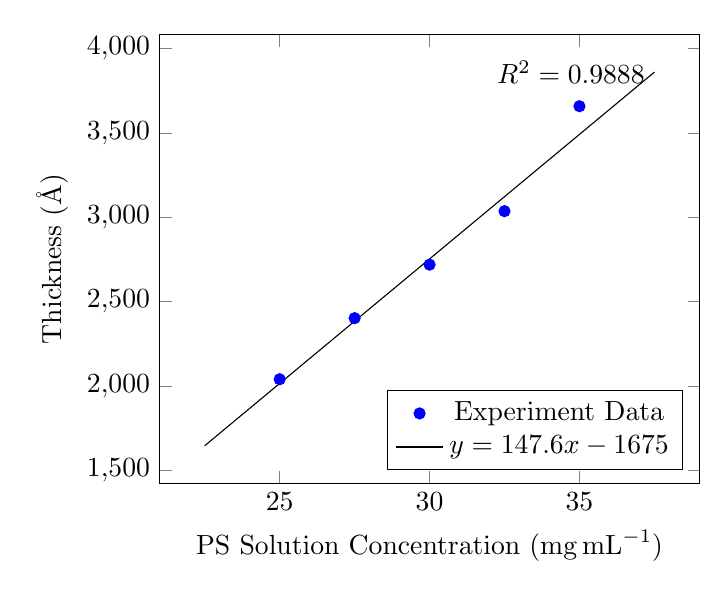
\begin{tikzpicture}
                            \begin{axis}[ 
                            xlabel={PS Solution Concentration (\unit{\milli\gram\per\milli\liter})},
                            ylabel={Thickness (\unit{\angstrom})},
                            legend pos=south east,
                            ] 
                            
                            \addplot [
                                color = blue,
                                fill = blue,
                                mark = *, % A filled circle
                                only marks
                            ] coordinates {
                                ( 25, 2040 )
                                ( 27.5, 2402 )
                                ( 30, 2719 )
                                ( 32.5, 3036 )
                                ( 35, 3658 )
                                };
                                \addlegendentry{Experiment Data}
                            \addplot[
                                color = black,
                                mark = none
                                ] coordinates {
                                ( 22.5, 1646 )
                                ( 37.5 , 3860 )
                                }
                                node [left] {$R^2 = 0.9888$};
                                \addlegendentry{$y = 147.6x -1675$}
                            \end{axis}
                        \end{tikzpicture}
                    \caption{Plot of polystyrene film thickness as measured by the ellipsometer.}\label{fig:ellips}
                \end{figure}

                \subsubsection{Calculations}

                In our investigation using the linear regression model, we have determined that the line of best fit can be expressed as $y = 147.6x - 1675$. By applying this equation to extrapolate the results to a thickness of 2000 \unit{\angstrom}, we calculated the critical concentration of polystyrene in toluene to be \qty{24.9}{\milli\gram\per\milli\liter}. Finally, we use the equation listed below where $x$ stands for the critical concentration, and $y$ stands for molecular weight\autocite{WOS:Sood}:

                \begin{align}
                    \ln{(M_\text{w})} &= \ln{(8.743 \times 10^{11})} + (- 4.802) \ln{C_\text{c}}\\
                    \ln{M_\text{w}} &= \ln{(8.742 \times 1011)} - 4.802 \ln{(24.90)} \nonumber\\
                    M_\text{w} &= e^{\ln{(8.742 \times 1011)} - 4.802 \ln{(24.90)}} \nonumber\\
                    M_\text{w} &= \qty{172608}{\atomicmassunit} \nonumber
                \end{align}

            \subsection{Goniometer}
                \begin{figure}
                    \centering
                    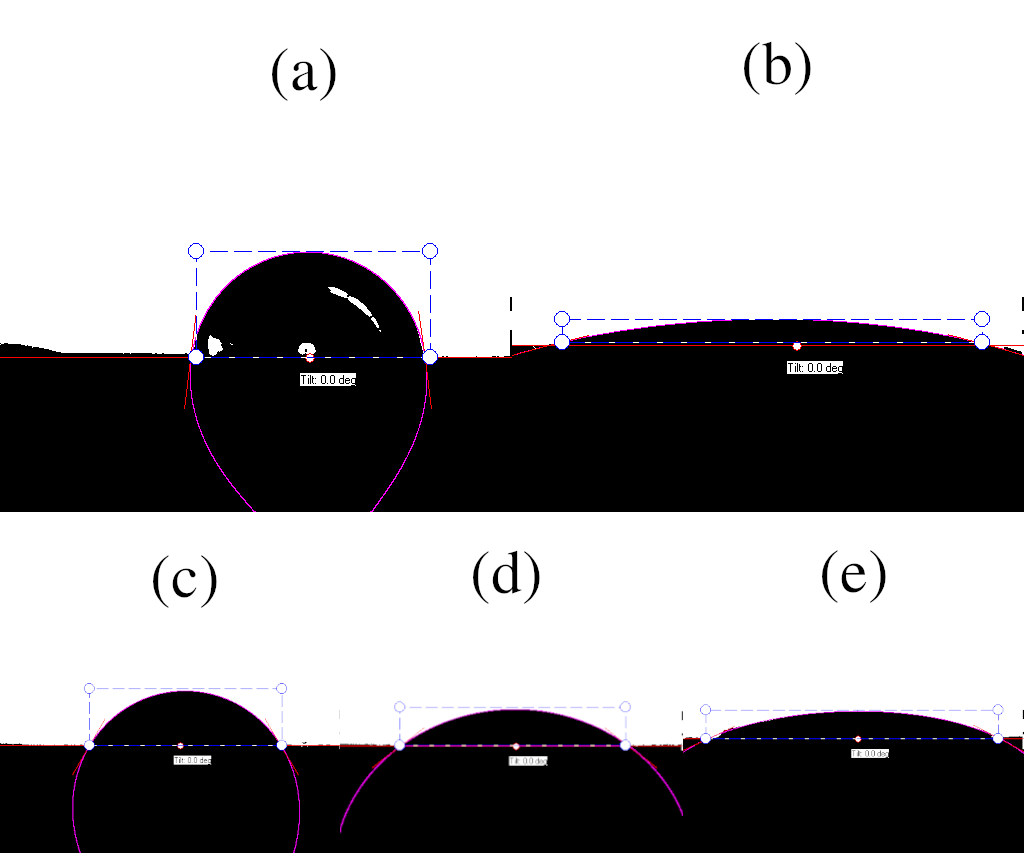
\includegraphics[width=0.8\columnwidth]{img/contact.png}
                    \caption{Water droplet contact angles. (a) was the Silicon wafer control; (b) was the Polystyrene 37.5 mg/mL control; (c), (d), and (e) were treated with UV light for 2 minutes, 3.5 minutes, and 5 minutes, respectively.}\label{fig:contact}
                \end{figure}
                To measure the contact angle, a single drop of distilled water was applied to several \qty{37.5}{\milli\gram\per\milli\liter} PS silicon wafer samples observed with the goniometer (Figure \ref{fig:contact}). The data obtained for the samples treated with varying time lengths of UV/ozone follows a predictable trend; as the exposure time to UV/ozone increased, the PS surface became more polarized, and the water droplet adhered to a greater area, leading to a lower contact angle. Hydrophilic surfaces have a contact angle of less than 90° while hydrophobic surfaces have a contact angle between 90° and 180°. The unaltered PS control sample had an average contact angle of 82°.

                \begin{table}
                    \centering
                    \begin{tabular}{@{}cccc@{}}
                        \toprule
                        Treatment                & Left (deg) & Right (deg) & Avg. (deg) \\ \midrule
                        Unaltered PS    & 82.98          & 82.05           & 82.52             \\
                        Si Wafer            & 14.66          & 15.58           & 15.12             \\
                        2 min UV/Ozone   & 59.99          & 59.36           & 59.68             \\
                        3.5 min UV/Ozone & 37.33          & 37.69           & 37.51             \\
                        5 min UV/Ozone   & 25.14          & 27.84           & 26.49             \\ \bottomrule
                        \end{tabular}
                    \caption{Left, right, and average contact angles obtained from contact angle goniometry.}\label{tab:contact}
                \end{table}
            
            \subsection{UV-Vis Spectroscopy}

                \begin{table*}
                    \centering
                    \begin{tabular}{@{}cc@{}}
                        \toprule
                        Concentration of PS 280K & Absorbance at 290 nm \\ \midrule
                        15                                & 0.026                \\
                        20                                & 0.015                \\
                        25                                & 0.039                \\
                        30                                & 0.156                \\
                        32.5                              & 0.071                \\
                        37.5                              & 0.129                \\ \bottomrule
                    \end{tabular}
                    \caption{Caption: Absorbance of PS solutions used at 290 nm.}\label{tab:abs}
                \end{table*}

                \begin{figure*}
                    \centering
                    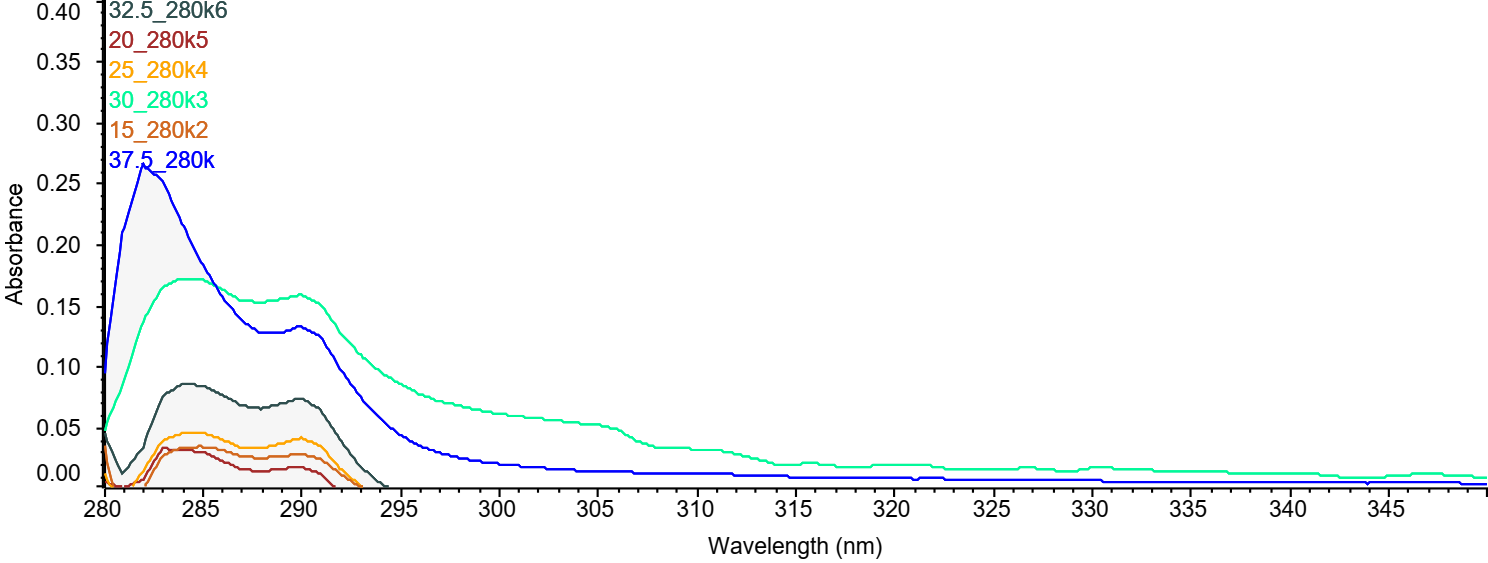
\includegraphics[width=0.8\textwidth]{img/uvvis.png}
                    \caption{Graph of UV-vis absorbance of solutions.}\label{fig:uv-vis}
                \end{figure*}
                To measure absorbance at \qty{290}{\nano\meter}, Beer Lambert Law of $A = lc$ is utilized. This equation states that absorbance and concentration are directly proportional to each other. Measuring absorbance ensures that all solutions made for spincasting are at the proper concentration. However, upon inspecting the levels of absorbance at \qty{290}{\nano\meter}, there is no distinct pattern of absorbance increase as concentration increases.
                
                Consequently, these unpredictable results indicate significant issues with the concentration of the solutions. This can most likely be attributed to the high concentration of polystyrene utilized in the solutions. The large amounts of  polystyrene were not properly dissolved into the solution, leading to inconsistencies in absorbance.                

            \subsection{Differencial Scanning Calorimeter}
                \begin{figure}[H]
                    \centering
                    \includegraphics[width=\columnwidth]{img/dsc.pdf}
                    \caption{DSC Heat flow data. Glass transition temperature of PS sample is 107.41°C.}\label{fig:dsc}
                \end{figure}
                Through the utilization of Differential Scanning Calorimetry (DSC) analysis, the glass transition temperature ($T_\text{g}$) of the polystyrene specimen was precisely ascertained to be \qty{107.41}{\degreeCelsius}. The glass transition phenomenon characterizes the temperature range at which the polymer undergoes a transition from a rigid state to a more flexible state, imparting significant insights into the nature of the molecular interactions within the material. 
                
                This transition is intrinsically linked to the intermolecular forces governing the polymer molecules\autocite{WOS:COUCHMAN}. The determination of the $T_\text{g}$ assumes paramount importance in confirming the molecular weight of the polystyrene sample, thereby contributing to a comprehensive understanding of its structural properties and behavior.

            \subsection{FTIR}
                \begin{figure}[H]
                    \centering
                    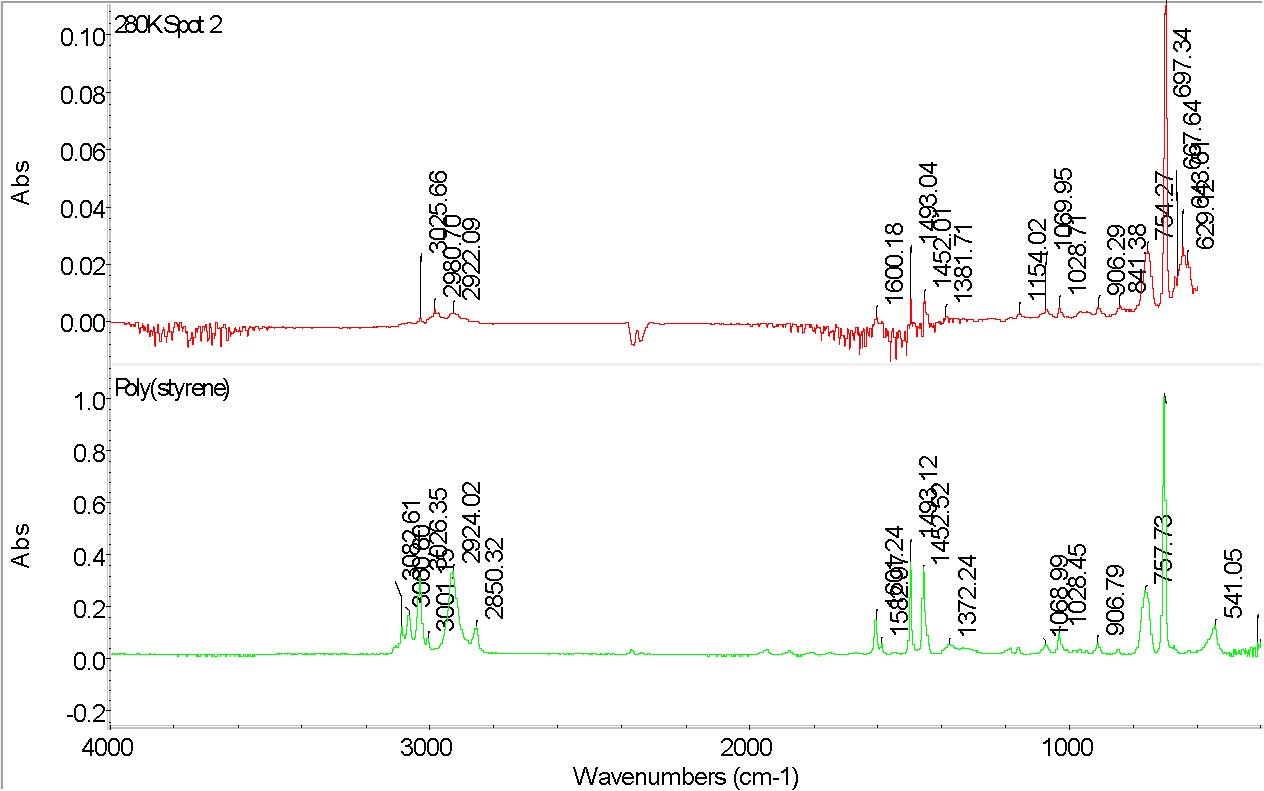
\includegraphics[width=\columnwidth]{img/ftir-comp.png}
                    \caption{FTIR absorbance vs wavenumbers, with sample spectrum in red and computer database spectrum in green.}\label{fig:ftir-comp}
                \end{figure}
                Using FTIR spectroscopy, a graph of wavenumber vs. absorbance  was generated. Because distinct  molecular bonds will absorb at different intensities and wavenumbers, the graph generated by FTIR serves as a fingerprint for sample identity. Figure \ref{fig:ftir-comp} demonstrates that our sample closely resembles the accepted FTIR spectrum for PS, with some negative absorbance noise that indicates discrepancies when subtracting out the base spectrum.
            
            \subsection{Keyence Microscopy}

            \begin{figure}
                \centering
                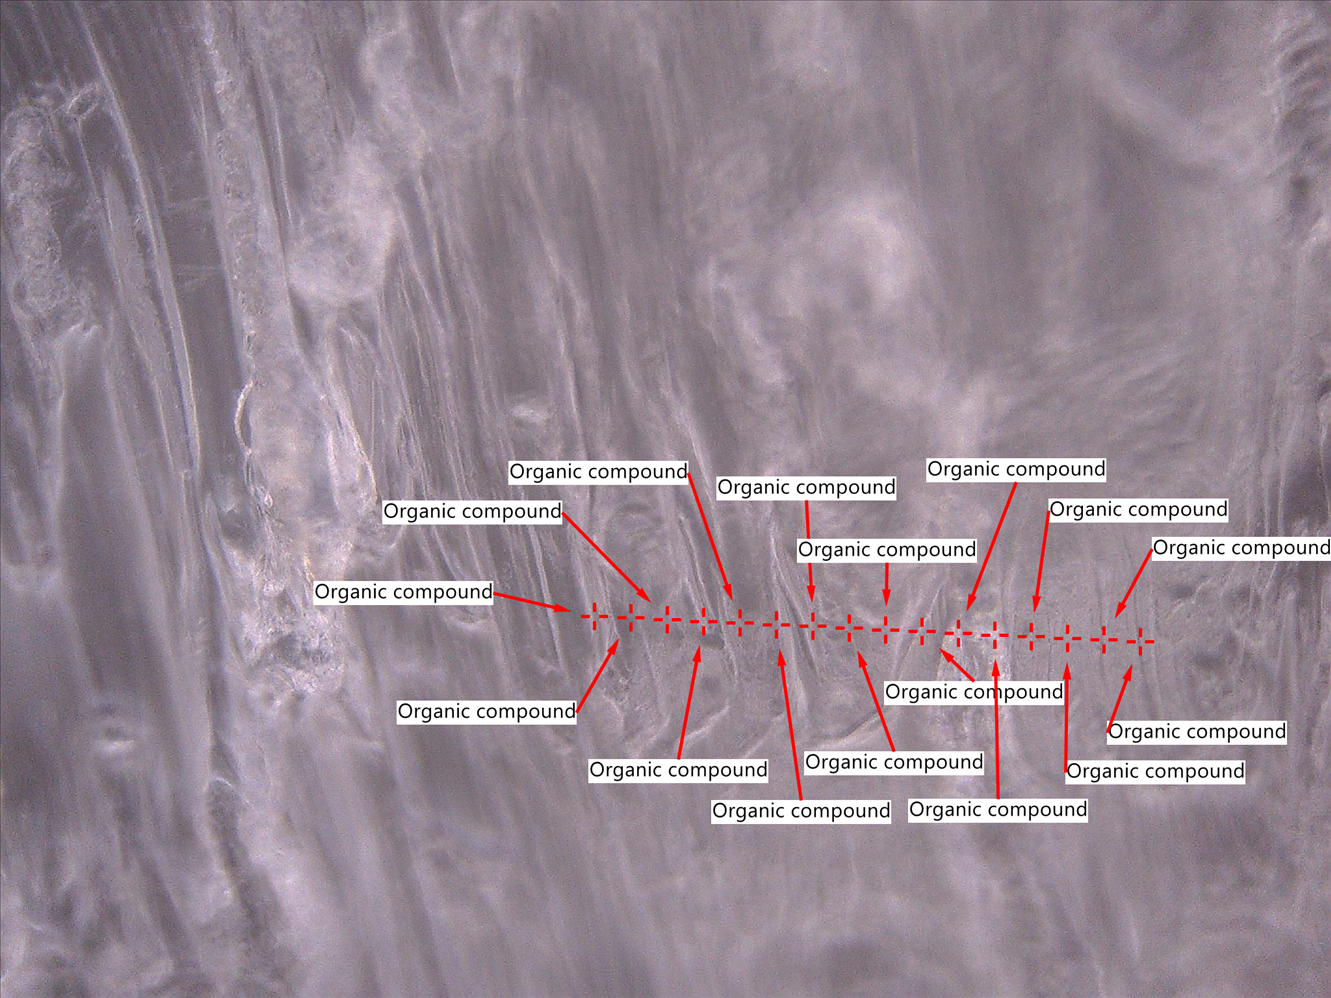
\includegraphics[width=\columnwidth]{img/keyence.png}
                \caption{Image captured via Keyence microscopy.}\label{fig:key}
            \end{figure}

            \begin{table}
                \centering
                \begin{tabular}{@{}cccccc@{}}
                    \toprule
                    No. & \multicolumn{2}{c}{Presumed material} & C      & H      & O     \\ \midrule
                    1   & \multicolumn{2}{c}{Organic compound}  & 57.6\% & 42.4\% &       \\
                    2   & \multicolumn{2}{c}{Organic compound}  & 54.7\% & 38.6\% & 6.7\% \\
                    3   & \multicolumn{2}{c}{Organic compound}  & 58.6\% & 41.4\% &       \\
                    4   & \multicolumn{2}{c}{Organic compound}  & 62.1\% & 37.9\% &       \\
                    5   & \multicolumn{2}{c}{Organic compound}  & 59.5\% & 40.5\% &       \\
                    6   & \multicolumn{2}{c}{Organic compound}  & 61.7\% & 38.3\% &       \\
                    7   & \multicolumn{2}{c}{Organic compound}  & 59.5\% & 35.0\% & 5.5\% \\
                    8   & \multicolumn{2}{c}{Organic compound}  & 61.7\% & 38.3\% &       \\
                    9   & \multicolumn{2}{c}{Organic compound}  & 56.1\% & 36.7\% & 7.2\% \\
                    10  & \multicolumn{2}{c}{Organic compound}  & 46.2\% & 46.3\% & 7.5\% \\
                    11  & \multicolumn{2}{c}{Organic compound}  & 61.0\% & 39.0\% &       \\
                    12  & \multicolumn{2}{c}{Organic compound}  & 53.1\% & 46.9\% &       \\
                    13  & \multicolumn{2}{c}{Organic compound}  & 63.4\% & 36.6\% &       \\
                    14  & \multicolumn{2}{c}{Organic compound}  & 60.7\% & 39.3\% &       \\
                    15  & \multicolumn{2}{c}{Organic compound}  & 62.9\% & 37.1\% &       \\
                    16  & Organic compound          &           & 64.3\% & 35.7\% &       \\ \bottomrule
                \end{tabular}
                \caption{Material analyses of Keyence image. Samples go from left to right in sequential order.}\label{tab:key}
            \end{table}

            \subsection{Error Propagation}
                \subsubsection{Concentration}
                    Error propagation was performed on the relationship $C$ (concentration) $=$ M (the mass of solute, polystyrene) divided by $V$ (the volume of the solvent, toluene). $dC$, the error of concentration $C$, can be found using the following formula for relationships involving multiplication or division: 
                    
                    \begin{equation}
                        \frac{dC}{C} = \sqrt{(\frac{dM}{M})^2 + (\frac{dV}{V})^2}
                    \end{equation}
                    
                    where $dM$ is the uncertainty of the mass $M$ of polystyrene upon weighing, $dV$ is the uncertainty of the volume $V$ of toluene upon pipetting, The uncertainty associated with the mass of polystyrene was \qty{\pm 0.01}{\milli\gram} ($dM = 0.01$), and the uncertainty associated with the volume of toluene was \qty{\pm 0.1}{\milli\liter} ($dV = 0.1$). 
                    \begin{align}
                        dC = 25\sqrt{(\frac{0.01}{69.9})^2 + (\frac{0.1}{2.80})^2} &= \pm \qty{0.893}{\milli\gram\per\milli\liter}\\
                        dC = 25\sqrt{(\frac{0.01}{72.9})^2 + (\frac{0.1}{2.62})^2} &= \pm \qty{1.050}{\milli\gram\per\milli\liter}\\
                        dC = 25\sqrt{(\frac{0.01}{87.7})^2 + (\frac{0.1}{2.92})^2} &= \pm \qty{1.027}{\milli\gram\per\milli\liter}\\
                        dC = 25\sqrt{(\frac{0.01}{95.1})^2 + (\frac{0.1}{2.93})^2} &= \pm \qty{1.109}{\milli\gram\per\milli\liter}\\
                        dC = 25\sqrt{(\frac{0.01}{98.8})^2 + (\frac{0.1}{2.83})^2} &= \pm \qty{1.237}{\milli\gram\per\milli\liter}\\
                        dC = 25\sqrt{(\frac{0.01}{101.6})^2 + (\frac{0.1}{2.71})^2} &= \pm \qty{1.384}{\milli\gram\per\milli\liter}
                    \end{align}
                    However, due to practical constraints, ellipsometry testing for the wafer coated with \qty{37.5}{\milli\gram\per\milli\liter} solution was not performed. Thus, the average $dC$ used for molecular weight calculations will be $\pm 1.063$

                \subsubsection{Molecular Weight}
                    \begin{align}
                        M_\text{w} &= y = \qty{172608}{\atomicmassunit} \nonumber\\
                        C &= \qty{24.9}{\milli\gram} \nonumber\\
                        dC &= 1.117 \nonumber\\
                        dy &= dM_\text{w} \nonumber
                    \end{align}
                    \begin{align}
                        \ln y &= \ln{(8.742 \times 10^{11})} - 4.802 \ln{C}\\
                        \frac{1}{y}dy &= \frac{-4.802}{C}dC \nonumber\\
                        dy &= \frac{-4.802 \times M_\text{w}}{C}dC \nonumber\\
                        dy &= \frac{-4.802 \times 172608 \times 1.117}{24.90} \nonumber\\
                        dM_\text{w} &= - 37182 \nonumber
                    \end{align}
                    \begin{align}
                        \text{Error} &= \frac{|dM_\text{w}|}{M_\text{w}} \times 100\%\\
                        \text{Error} &= 21.54\% \nonumber
                    \end{align}

        \section{Conclusion}
            This experiment was designed to evaluate the viability of determining the molecular weight of an unknown sample of PS by measuring a known PS sample ($M_\text{w} = 280K$) using spin-casting and ellipsometry. FTIR spectroscopy performed on the PS sample closely resembles standard PS FTIR data. DSC was performed and the experiment glass-transition temperature of \qty{107.41}{\degreeCelsius} was obtained, which closely matches current literature. Goniometry analysis of spun-cast films of the sample, which demonstrated low wettability, agreeing with knowledge that PS films are hydrophobic.

            Ellipsometry experiments, due to practical constraints, were done only once for each sample. This resulted in a relatively larger margin of error than originally proposed ($20.50\%$). 
            
            The results of this experiment could be significantly strengthened (and the margin of error drastically reduced) by minimizing the amount of human, systemic, and instrumentation error, as well as repeating individual measurements. For the ellipsometry data, more care could have gone into making sure the sample was better dissolved before being applied on the Si wafer, which would reduce human error. More careful handling of both uncoated and coated Si wafers, increased measurements taken from the ellipsometer, and more detailed experimental planning would greatly improve the reliability of our results.

            Altogether, the experiment reaffirms the viability of using spin-casting as a means to quickly estimate the molecular weight of polystyrene polymers.

        \section{Acknowledgements}
            The authors thank the Garcia Center for Polymers at Engineered Interfaces: Dr.~Rafailovich, Dr.~Cuiffo, Dr.~Sokolov, and Ms.~Hofflich for their support and mentorship over the course of this research; REUs Alex~Samadi, Jacob~Zerykier, Ruth~Pereira, and Milana~Stein for their guidance and supervision; and many other Stony Brook University faculty and students for their knowledge, expertise, and kindness. 
        \printbibliography
\end{document}
